\documentclass[conference]{IEEEtran}
\IEEEoverridecommandlockouts
% The preceding line is only needed to identify funding in the first footnote. If that is unneeded, please comment it out.
\usepackage{cite}
\usepackage{amsmath,amssymb,amsfonts}
\usepackage{algorithmic}
\usepackage{graphicx}
\usepackage[utf8]{inputenc}

% for romanian language
\usepackage[romanian]{babel}
\usepackage{textcomp}
\usepackage{xcolor}

% for code snippets
\usepackage{listings}	
\def\BibTeX{{\rm B\kern-.05em{\sc i\kern-.025em b}\kern-.08em
    T\kern-.1667em\lower.7ex\hbox{E}\kern-.125emX}}




\begin{document}

\title{Generarea imaginilor pe baza emoțiilor dintr-un text folosind Rețele Neuronale Adversariale și tehnici de interpretare a limbajului natural\\
{\footnotesize \textsuperscript{*}Work in Progress}
}

\author{
	\IEEEauthorblockN{1\textsuperscript{st} Paul-Cosmin Petrila
	}
		\IEEEauthorblockA{
		\textit{Facultatea de Automatică și Calculatoare} \\
		\textit{Specializarea Ingineria Sistemelor} \\
		\textit{Departamentul de Informatica Aplicat} \\
		\textit{Universitatea Tehnică ”Gheorghe Asachi”\\
		Iași, România \\
		petrila.paulcosmin@gmail.com}
	}
	\and\IEEEauthorblockN{2\textsuperscript{nd} Lavinia-Eugenia Ferariu}
	\IEEEauthorblockA{
		\textit{Facultatea de Automatică și Calculatoare} \\
		\textit{Specializarea Ingineria Sistemelor} \\
		\textit{Departamentul de Informatica Aplicat} \\
		\textit{Universitatea Tehnică ”Gheorghe Asachi”}\\
		Iași, România \\
		lavinia-eugenia.ferariu@academic.tuiasi.ro 
	}
}



\maketitle
\begin{abstract}
	In ultimii ani, detectarea emoțiilor în text a devenit din ce în ce mai populară
	datorită potențialului vast și aplicațiilor pe care îl are în marketing,
	psihologie, inteligență artificială etc. Accesul larg asupra cantităților mari de date tip text,
	mai ales texte cu opinii și sentimente puternice,
	a făcut posibilă antrenarea de modele de limbaj din ce în ce mai performante și credibile.
	De asemeni, generarea imaginilor folosind texte prin modele precum DALL-E \cite{dalle}.

	Această lucrare științifică își propune explorarea metodelor de analizare a sentimentelor 
	limbajului natural și generarea unor imagini corespondente acestor sentimente. 
	Analiza sentimentelor dintr-un text este îndeplinită utilizând BERT (Bidirectional Encoder Representations from Transformers)\cite{devlin2019bert},
	Pe baza rezultatului indicat de către LLM, rețeaua Conditional GAN va genera pentru fiecare text o imagine corespunzătoare. 

	
\end{abstract}

\begin{IEEEkeywords}
BERT, NLP, GAN, AI, LLM,
\end{IEEEkeywords}


\section{Introducere}

Detectarea emoțiilor în lingvistica computatională este procesul de identificare a emoțiilor 
discrete exprimate în text. Analiza emoțiilor poate fi privită ca o evoluție naturală a analizei 
sentimentelor și a modelului său mai detaliat. 
Cu toate acestea, așa cum observăm în acest articol, 
acest domeniu mai are mult de parcurs înainte de a egala succesul 


Domeniul inteligenței artificiale generative, bazat pe modele de limbaj de mari dimensiuni 
( Large Language Models - LLMs ) a avut parte de schimbări mari în ultimii ani. 
LLM-urile au devenit suficient de avansate încât pot fi folosite la un nivel mare
atât de companiile software, cât și de echipele de marketing, dar și în viața de zi cu zi a studenților și oamenilor obișnuiți. 


Astfel, prin metodele descrise mai în detaliu mai jos, sistemul de față îndeplinește următoarele criterii:
\begin{itemize}
	\item Procesează la intrare un text 
	\item Îl clasează într-o categorie de emoție
	\item Trimite răspunsul mai departe ca intrarea la generatorul C-GAN 
	\item Afișează o imagine generată pe baza sentimentului transmis
\end{itemize}


\section{Concepte de bază în Învățarea Automată și Inteligența Artificială}
Învățarea Automată (IA) reprezintă o ramură a inteligenței artificiale care se ocupă cu dezvoltarea sistemelor și 
algoritmilor capabili să învețe și să îmbunătățească performanța pe baza experienței.

\subsection{Cum definim inteligența artificială}
It is the science and engineering of making intelligent machines, especially intelligent computer programs. It is related to the similar task of using computers to understand human intelligence, but AI does not have to confine itself to methods that are biologically observable.
\subsection{Istoria dezvoltării Inteligenței Artificiale}

\subsection{Tipuri de inteligență artificială și problemele pe care le rezolvă}

%%%%%%%%%%%%%%%%
%%%%%%%%%%%%%%%
\section{Analiza emoțiilor dintr-un text }
Înțelegerea sentimentelor dintr-un text oferă companiilor care integrează astfel de soluții 
în cadrul aplicațiilor lor 
\subsection{Diferența dintre analiza sentimentelor și a emotiilor}
Analiza sentimentelor reprezintă un proces de categorizare a unui text drept pozitiv, negativ sau neutru.
Această polaritate a textului poate fi folosită pentru a obține o înțelegere de suprafață a textului,
fără, însă, a intra în detalii când vine vorba despre emoția trăită de cel care a scris textul.
Aplicațiile acestei metode includ: colectarea recenziilor unui produs și monitorizarea conținutului de 
pe rețelele de socializare \cite{mc90} .

Analiza emoțiilor, pe de altă parte, implică identificarea și categorizarea emoțiilor specifice exprimate prin text.
Se concentrează pe emoții mai specifice precum nostalgia, furia, frica, tristețea și bucuria, emoții trăite de autor 
în timp ce scria textul. Aplicațiile analizei de emoții includ: 
categorizarea interacțiunilor cu departamentul de relații cu clienții, sănătate mentală, crearea de conținut 
prin care se caută un anumit impact emoțional.


\subsection{Etichetarea textelor}
Cunoscută în Engleză drept Text Labeling, etichetarea textelor este foarte practicată și constituie
baza oricărei lucrări care își propune o problemă de identificare.
Există o mulțime de resurse online care oferă seturi de date deja etichetate.
Câteva exemple includ: Swiss Center for Affective Sciences (SCA), ISEAR ( International Survey On Emotion Antecedents And Reactions).

\subsection{Word Embedding}
Word Embedding este o tehnică de modelare semantică înrădăcinată în ideea următoare:
cuvintele care sunt folosite des împreună sunt similare într-un criteriu semnatic.
În acest tip de metode, fiecare cuvânt este reprezentat ca un vector într-un spațiu de dimensiune n,
numit spațiu vectorial, în care distanța dintre vectori corespunde cu similaritatea lor semantică.



%%%%%
%%%%%


\section{Arhitectura și funcționarea soluției dezvoltate}

\subsection{Arhitectura BERT}

\subsection{Arhitectura C-GAN}




%%%%%%%%%%
\section{Subiecte de abordat în continuare}
În următorul semestru voi realiza legătura dintre cele două modele cu care am lucrat.
Voi implementa niste comparatii intre GPT si BERT.
O interfata grafica pentru interactionarea cu programul scris de mine in python
probabil sub forma unei aplicatii web folosind tehnlogii de ultima generatie.
Implementarea ca serviciu Docker a scriptului de python pentru deployment
Detalierea mediului de lucru si uneltelor folosite ( latex, python etc )
Ce am invatat in urma folosirea acestor unelte.

\section{Planificare Activități}
\begin{itemize}
	\item Ianuarie 
	\item Februarie
	\item Martie
	\item Aprilie
\end{itemize}



\begin{figure}[htbp]
\centerline{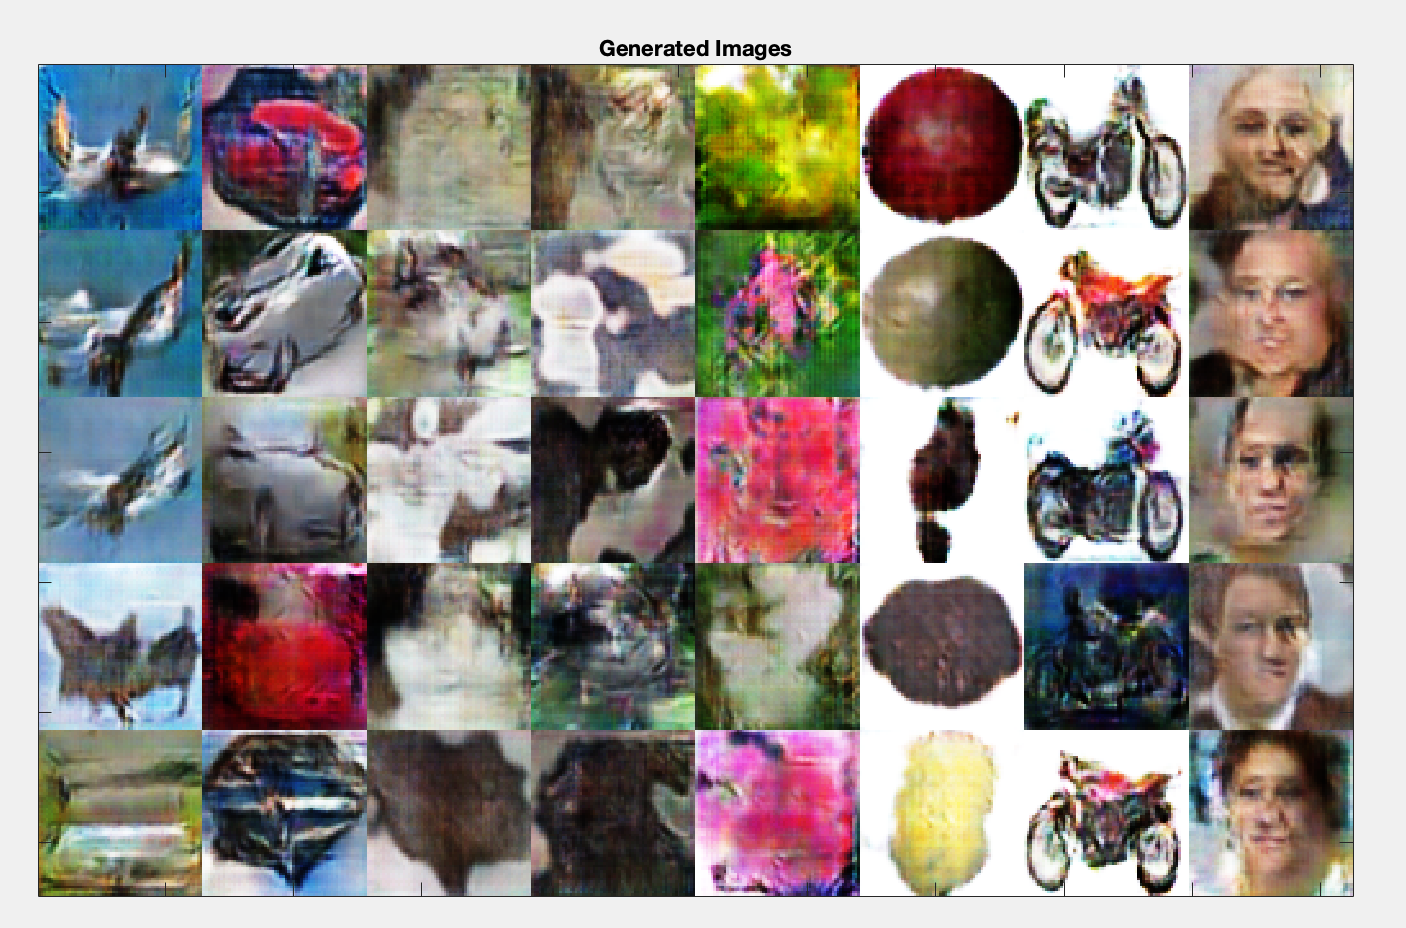
\includegraphics[width=0.5\textwidth]{fig1.png}}
\caption{Exemplu de imagine generată de modelul matlab.}
\label{fig}
\end{figure}


% \begin{thebibliography}{00}
% \end{thebibliography}
% \vspace{12pt}
\nocite{*}

\bibliographystyle{IEEEtran}
\bibliography{references}
\end{document}
